\documentclass[10pt,a4paper]{article}
\usepackage[utf8]{inputenc}
\usepackage[T1]{fontenc}
\usepackage{amsmath}
\usepackage{amssymb}
\usepackage{graphicx}
\usepackage[left=1cm,right=1cm,top=1cm,bottom=1cm]{geometry}
\begin{document}
	
	
	\textbf{Thème:}Calibrage/étalonnage de caméra et application à l’estimation de
	performances lors de sauts en longueur 
	
	
	\begin{center}
		\textbf{Feuille de route}
	\end{center}
	
	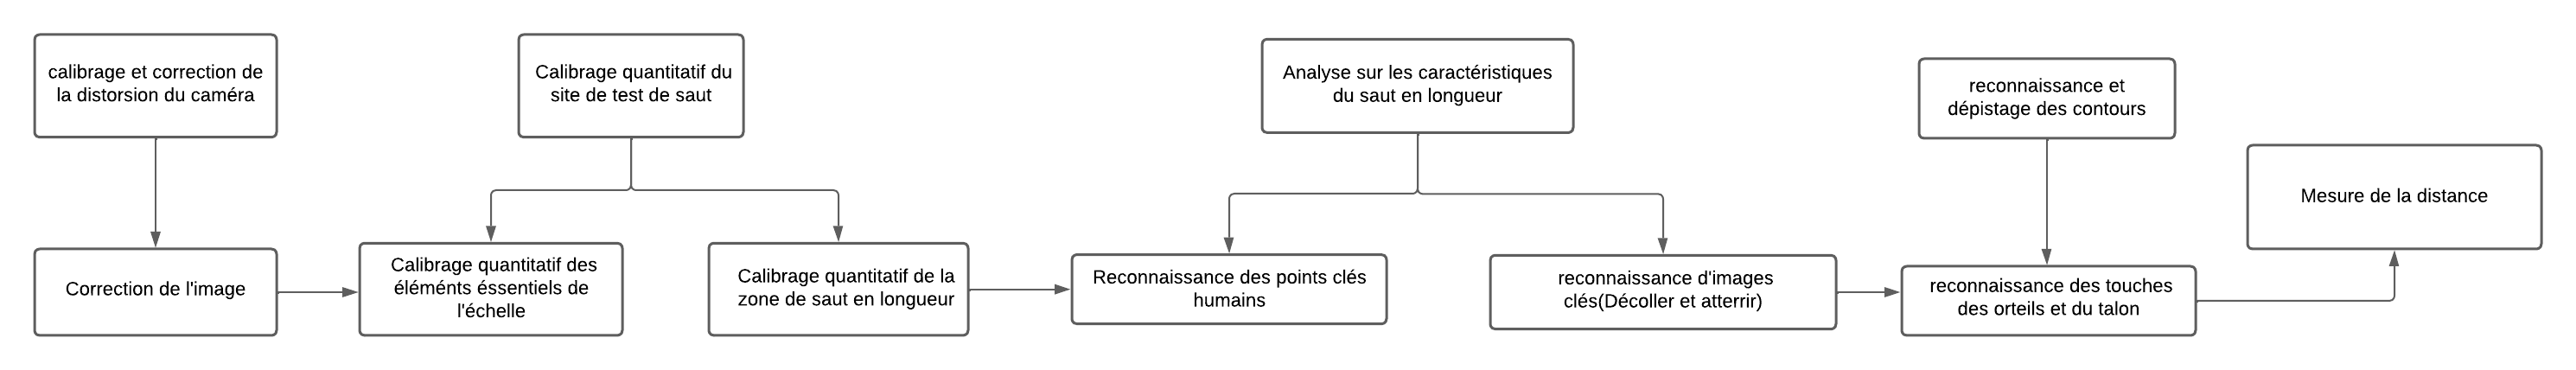
\includegraphics[scale=0.40]{image/Feuille de route}\\
	
	
\textbf{Les équipement à utilisés}	
	
\begin{itemize}
	\item Ordinateur portable\\
	
	\item Un échiquier \\
	
	\item Un raspberry Pi 3\\
	
	\item Un webcam ordinaire de résolution des pixels 1280 × 720 et une fréquence d'acquisition : 30 Hz \\
	
	\item Tapis de saut en longueur :340cm de long et 90cm de largeur\\
	
	\item Station d'accueil pour carte graphique externe de carte graphique 8g rtx-2070gpu \\
	
	\item Règle faite maison dont la largeur unitaire de chaque échelle est de 5 cm et la longueur totale	est de 3M.\\
	
	\item deux rubans rouges de 75 cm de long ; 4 cm de large
\end{itemize}	
	
	
	
	
	
	
	\begin{center}
		\textbf{Quelques questions}
	\end{center}
	
\begin{itemize}
	\item Quel images donne une caméras non calibré
	\item donner une notion sur la vision par ordinateur,l'intelligence artificiel et la télémétrie\\
	
	\item Rechercher l'algorithme ou le logiciel de zhang 
\end{itemize}	
	
	
	
\end{document}